\begin{table}[H]
\fontsize{8}{12}\selectfont
\caption{Requisitos de usuário}
\resizebox{\textwidth}{!}{%
\begin{tabular}{p{0.7cm}p{8cm}}
{[}RU01{]} & O sistema deverá permitir login dos administradores através do Facebook ou usando e--mail e senha do usuário cadastrados, autorizando que acessem ao sistema e nele realize as funções permitidas. \\
{[}RU02{]} & O sistema deverá permitir que o usuário devidamente cadastrado consiga criar publicações. \\
{[}RU03{]} & O sistema deverá permitir que o usuário devidamente cadastrado consiga editar as publicações que foram criadas. \\
{[}RU04{]} & O sistema deverá permitir que o usuário devidamente cadastrado consiga excluir uma ou mais publicações criadas. \\
{[}RU05{]} & O sistema deverá confirmar se o usuário deseja excluir uma publicação. \\
{[}RU06{]} & O sistema deverá listar todas as publicações criadas. \\
{[}RU07{]} & O sistema deverá armazenar todas as informações que forem inseridas para que possam serem feitas as edições, listagens e exclusões. \\
{[}RU08{]} & O sistema deverá possuir uma página de acesso público. \\
{[}RU09{]} & O sistema deverá apresentar apenas as publicações e comentários autorizados. \\
{[}RU10{]} & O sistema deverá possuir internet conectada. \\
{[}RU11{]} & O sistema deverá funcionar nos navegadores de internet dos sistemas operacionais Linux, Windows.
\end{tabular}%
}
\end{table}

\begin{figure}
    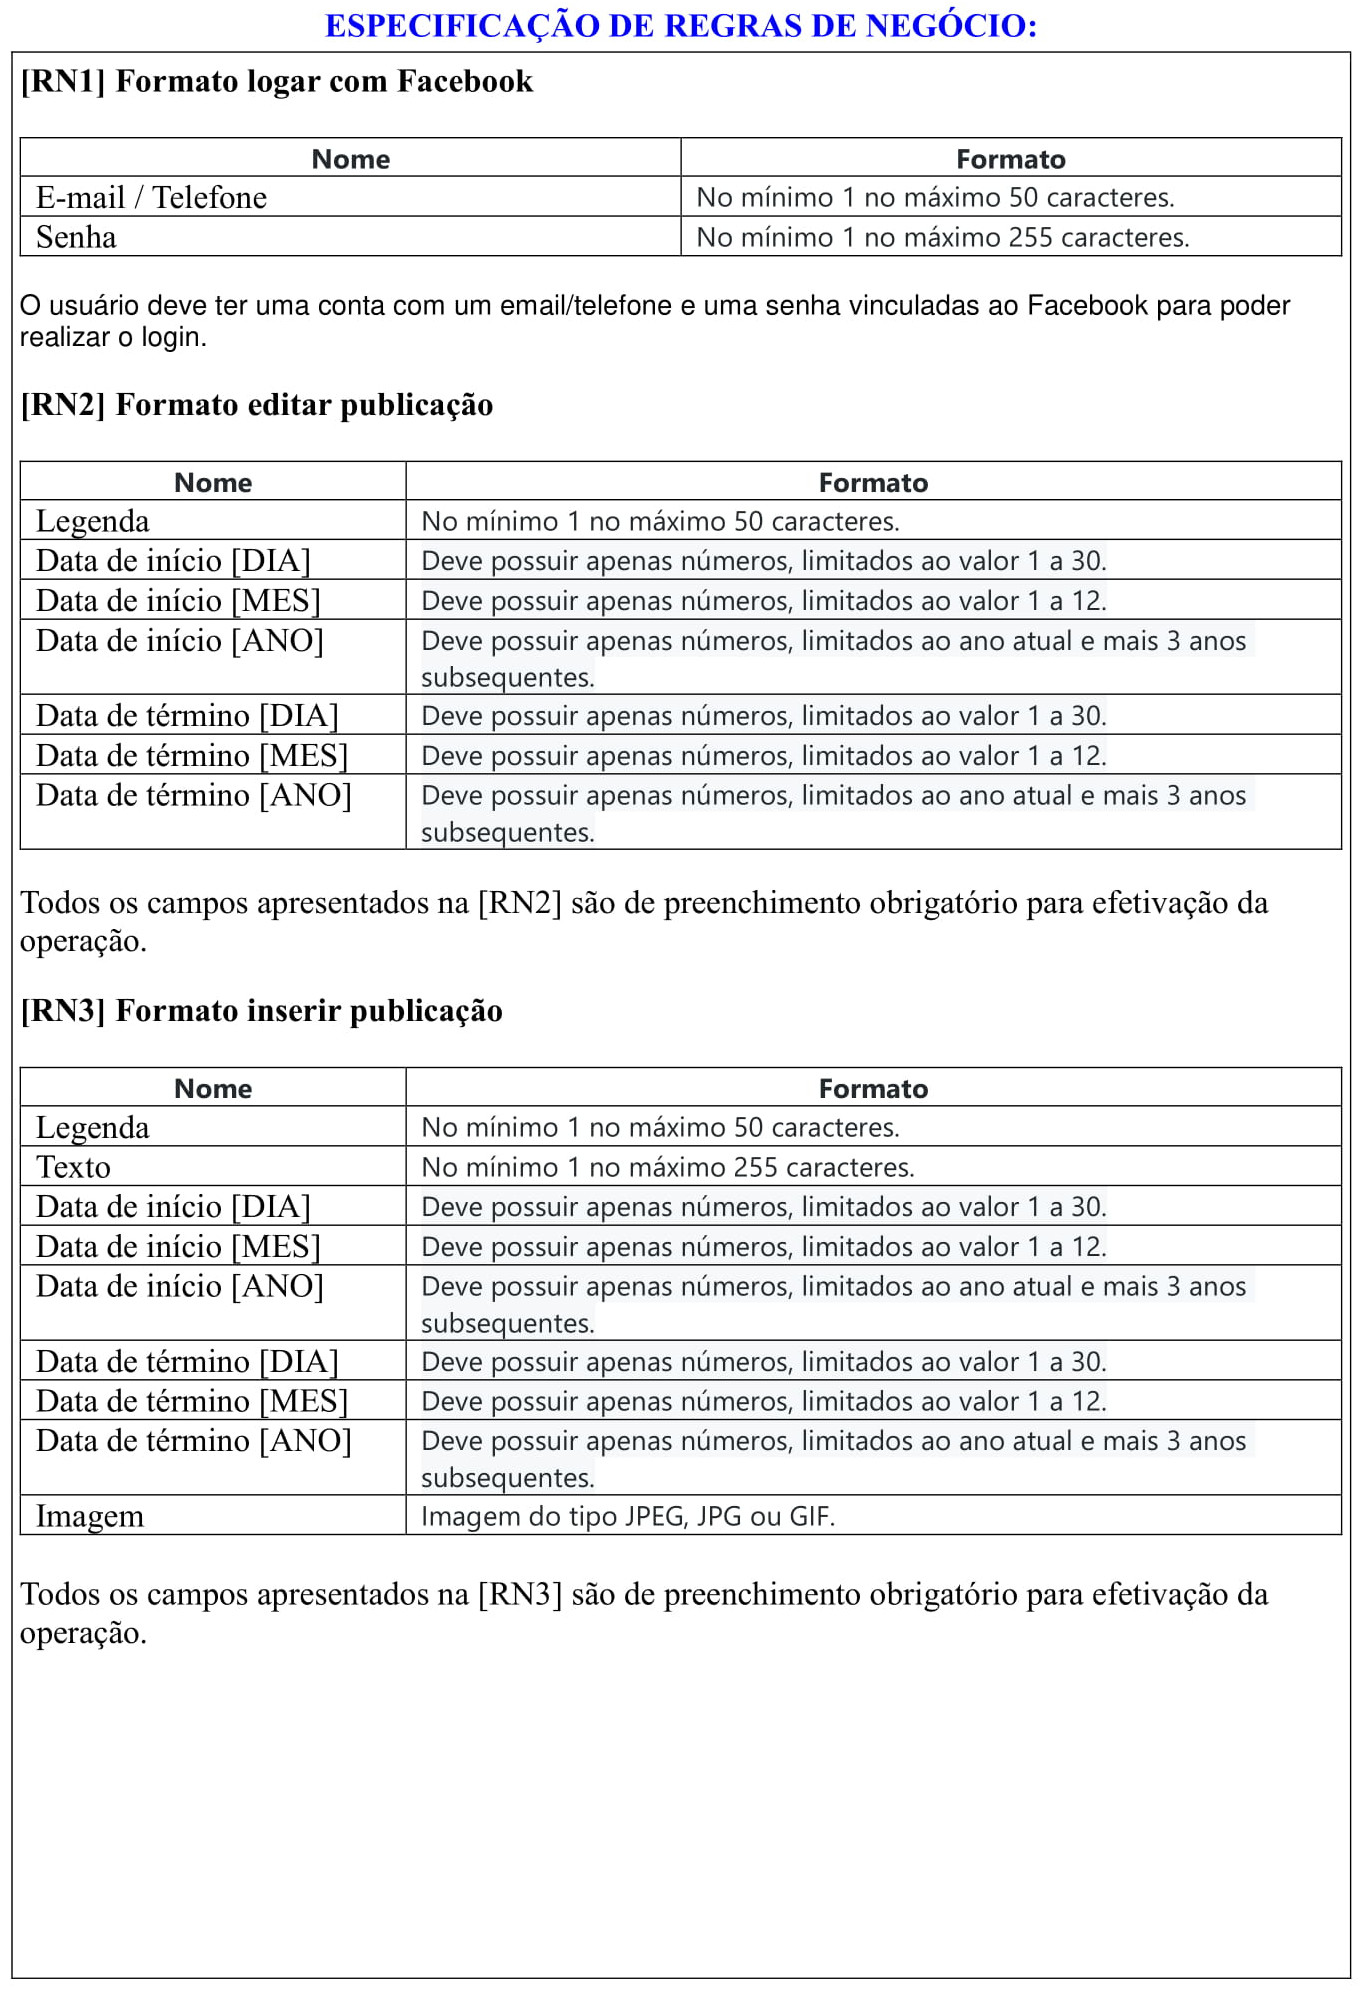
\includegraphics[width=\textwidth]{documentacao/ModeloArtefatos-01.jpg}
\end{figure}

\begin{figure}
    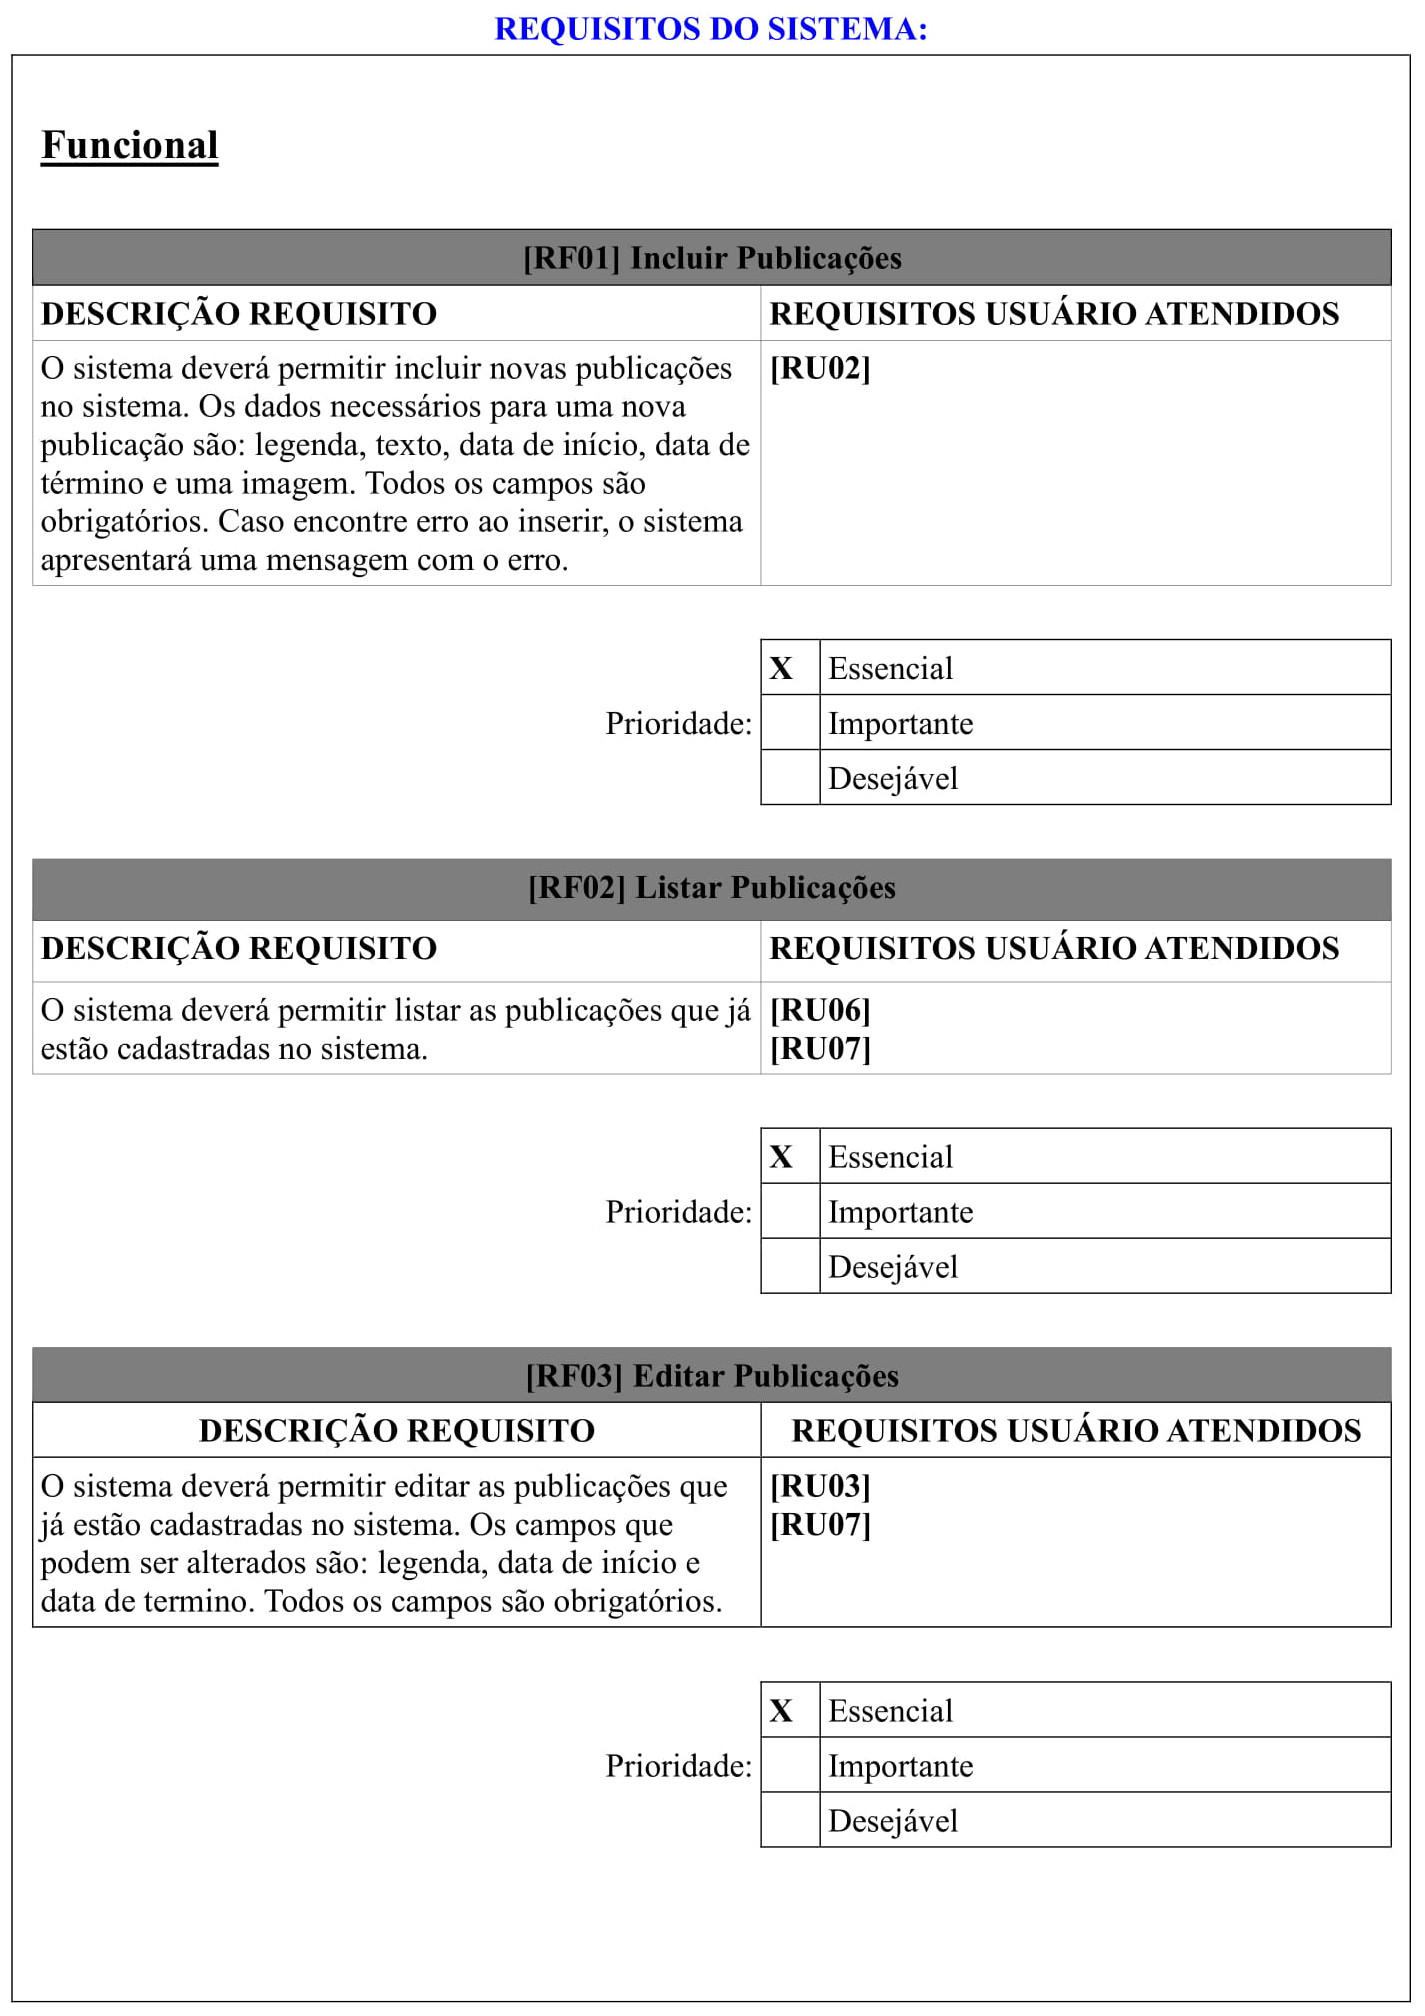
\includegraphics[width=\textwidth]{documentacao/ModeloArtefatos-02.jpg}
\end{figure}

\begin{figure}
    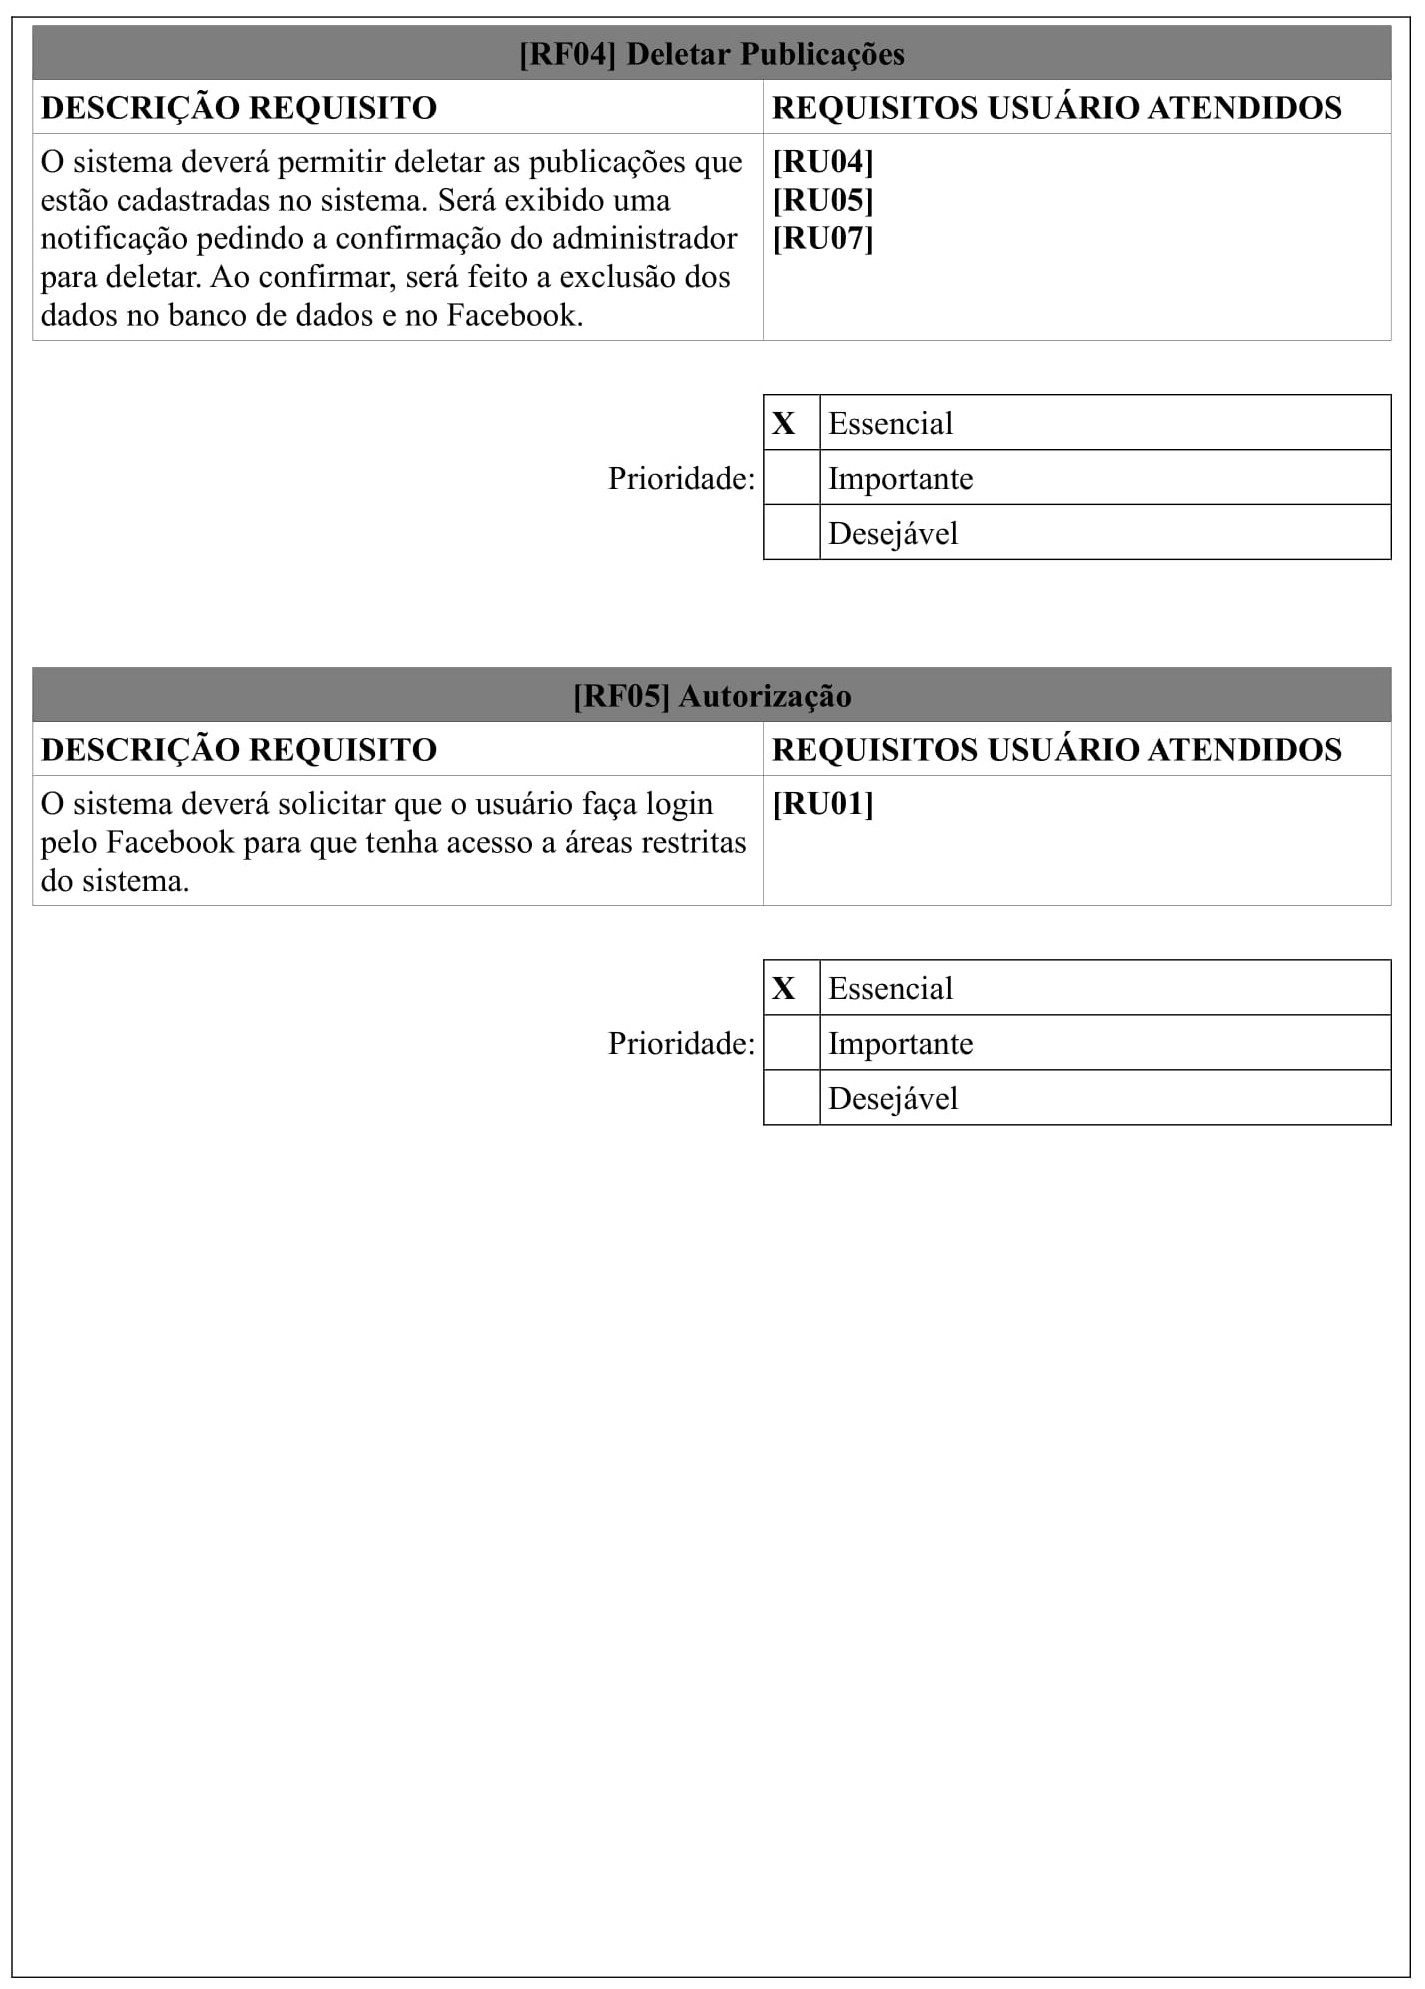
\includegraphics[width=\textwidth]{documentacao/ModeloArtefatos-03.jpg}
\end{figure}

\begin{figure}
    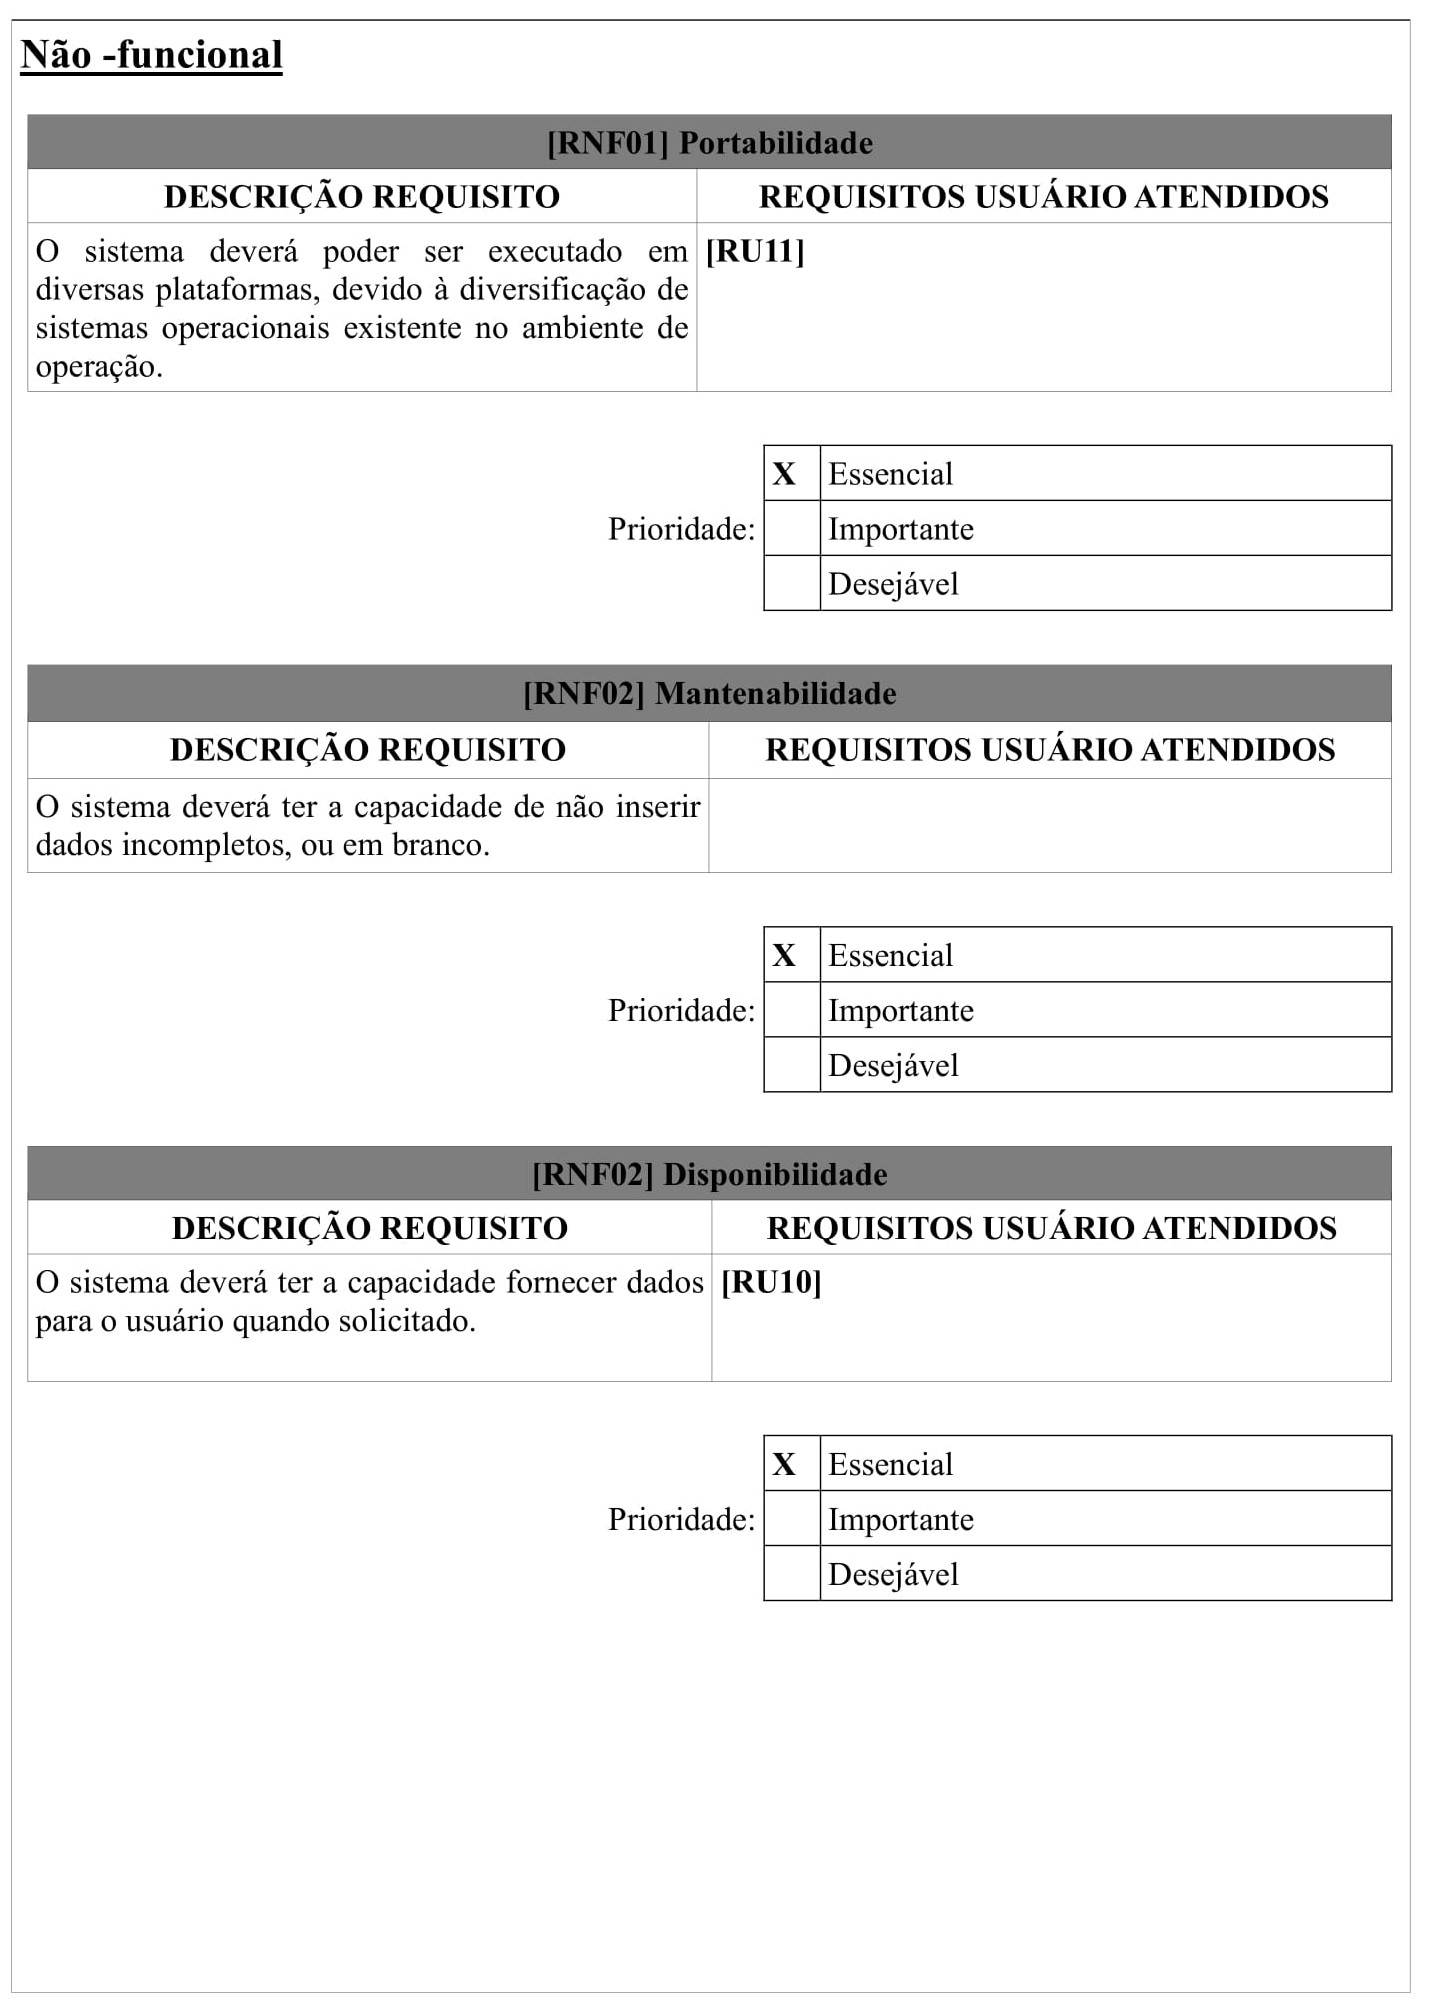
\includegraphics[width=\textwidth]{documentacao/ModeloArtefatos-04.jpg}
\end{figure}

\begin{figure}
    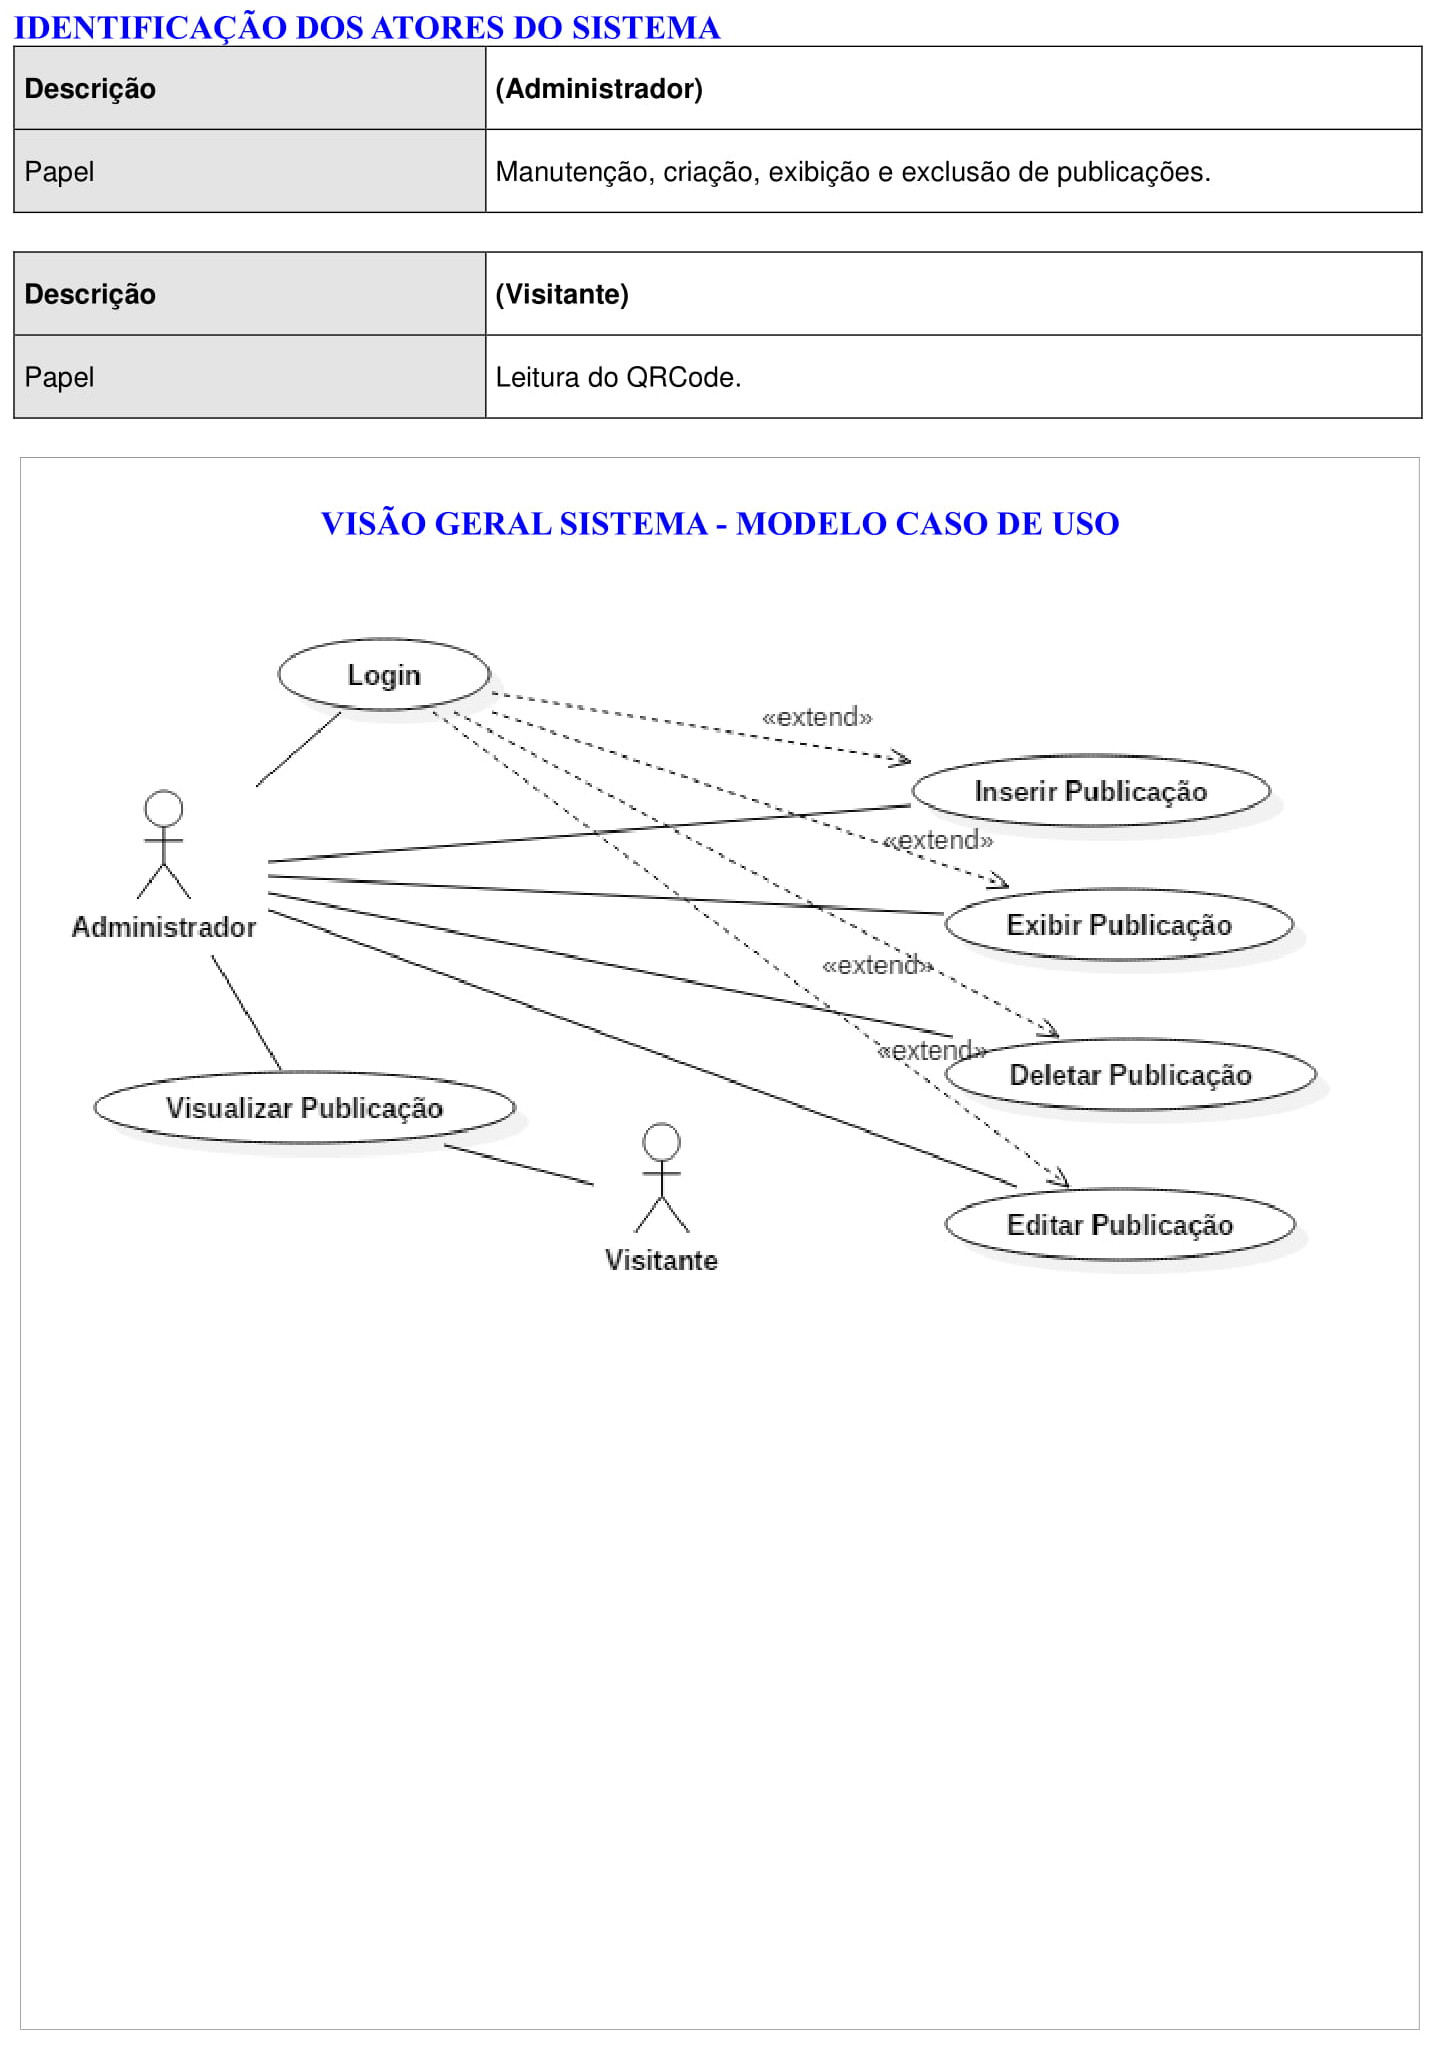
\includegraphics[width=\textwidth]{documentacao/ModeloArtefatos-05.jpg}
\end{figure}

\begin{figure}
    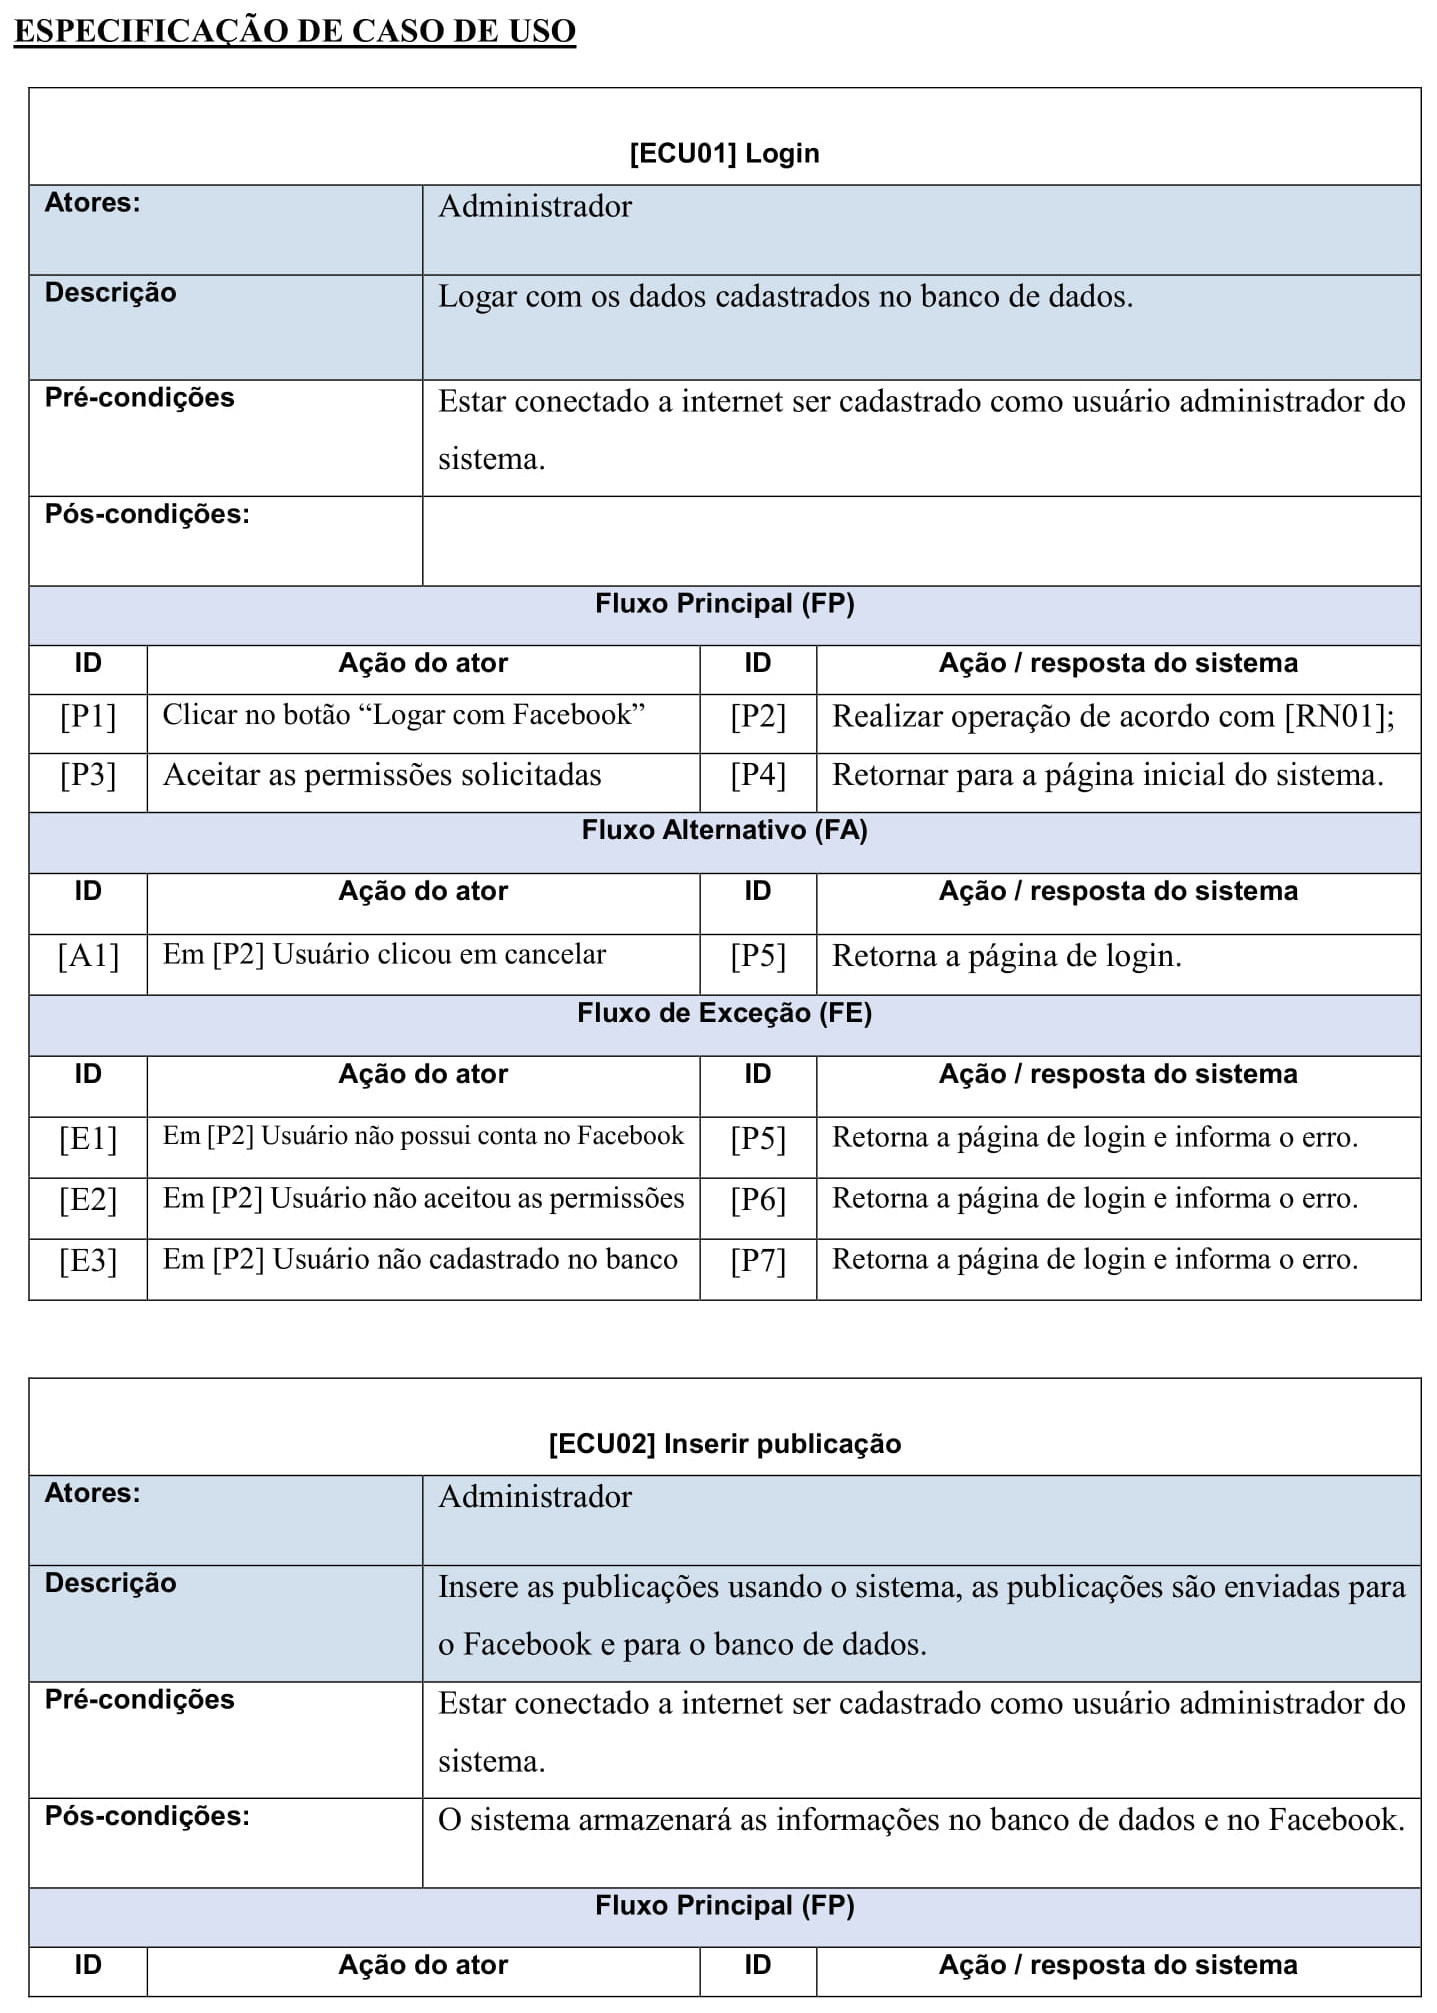
\includegraphics[width=\textwidth]{documentacao/ModeloArtefatos-06.jpg}
\end{figure}

\begin{figure}
    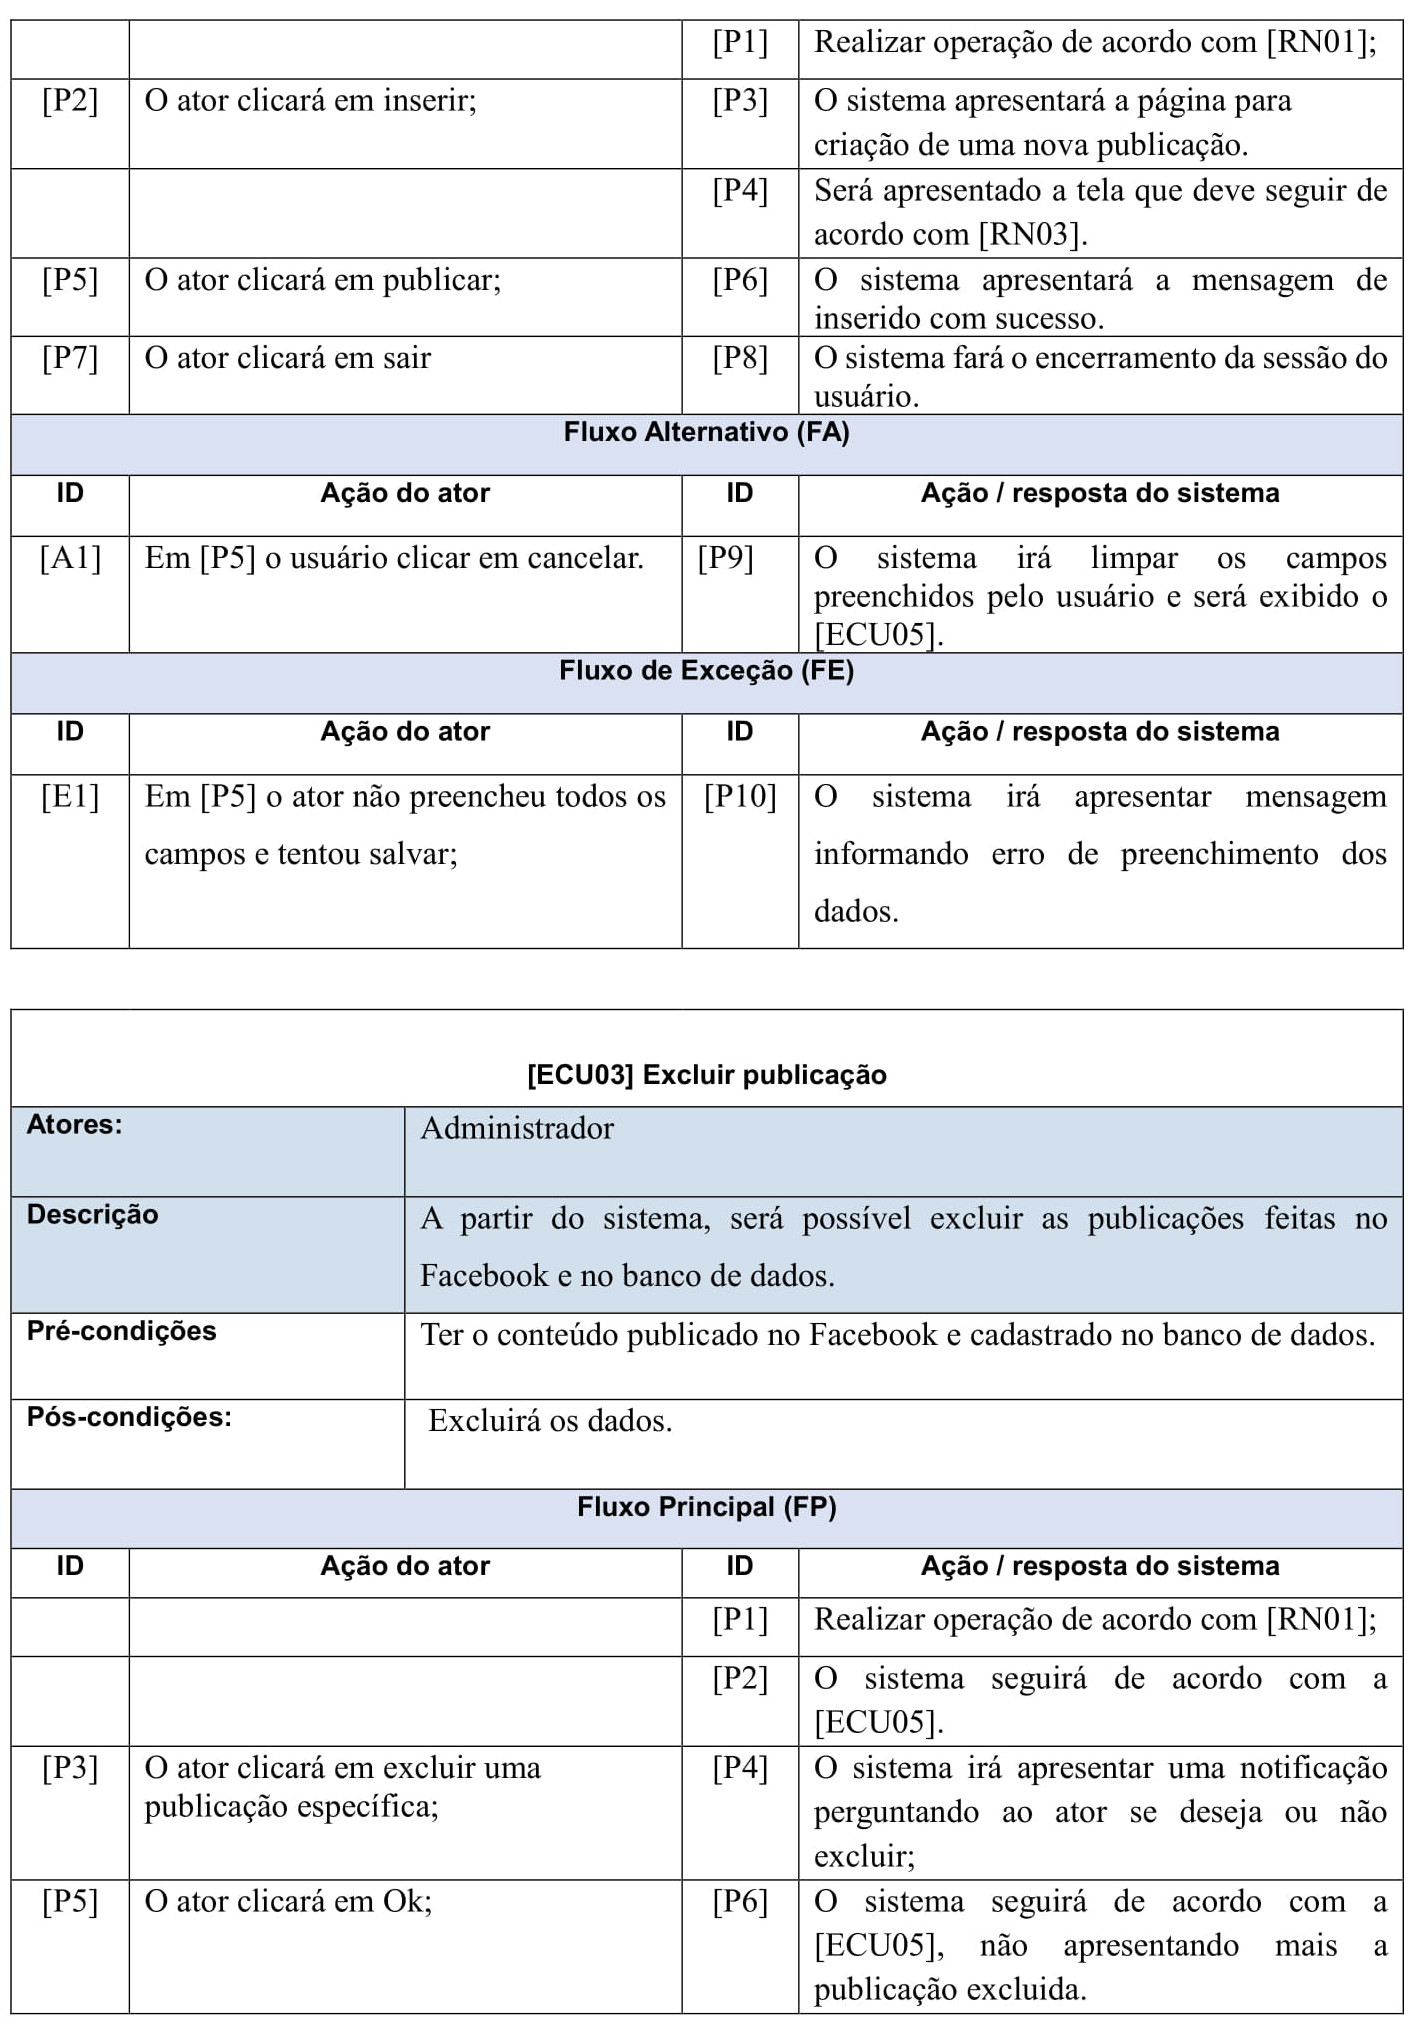
\includegraphics[width=\textwidth]{documentacao/ModeloArtefatos-07.jpg}
\end{figure}

\begin{figure}
    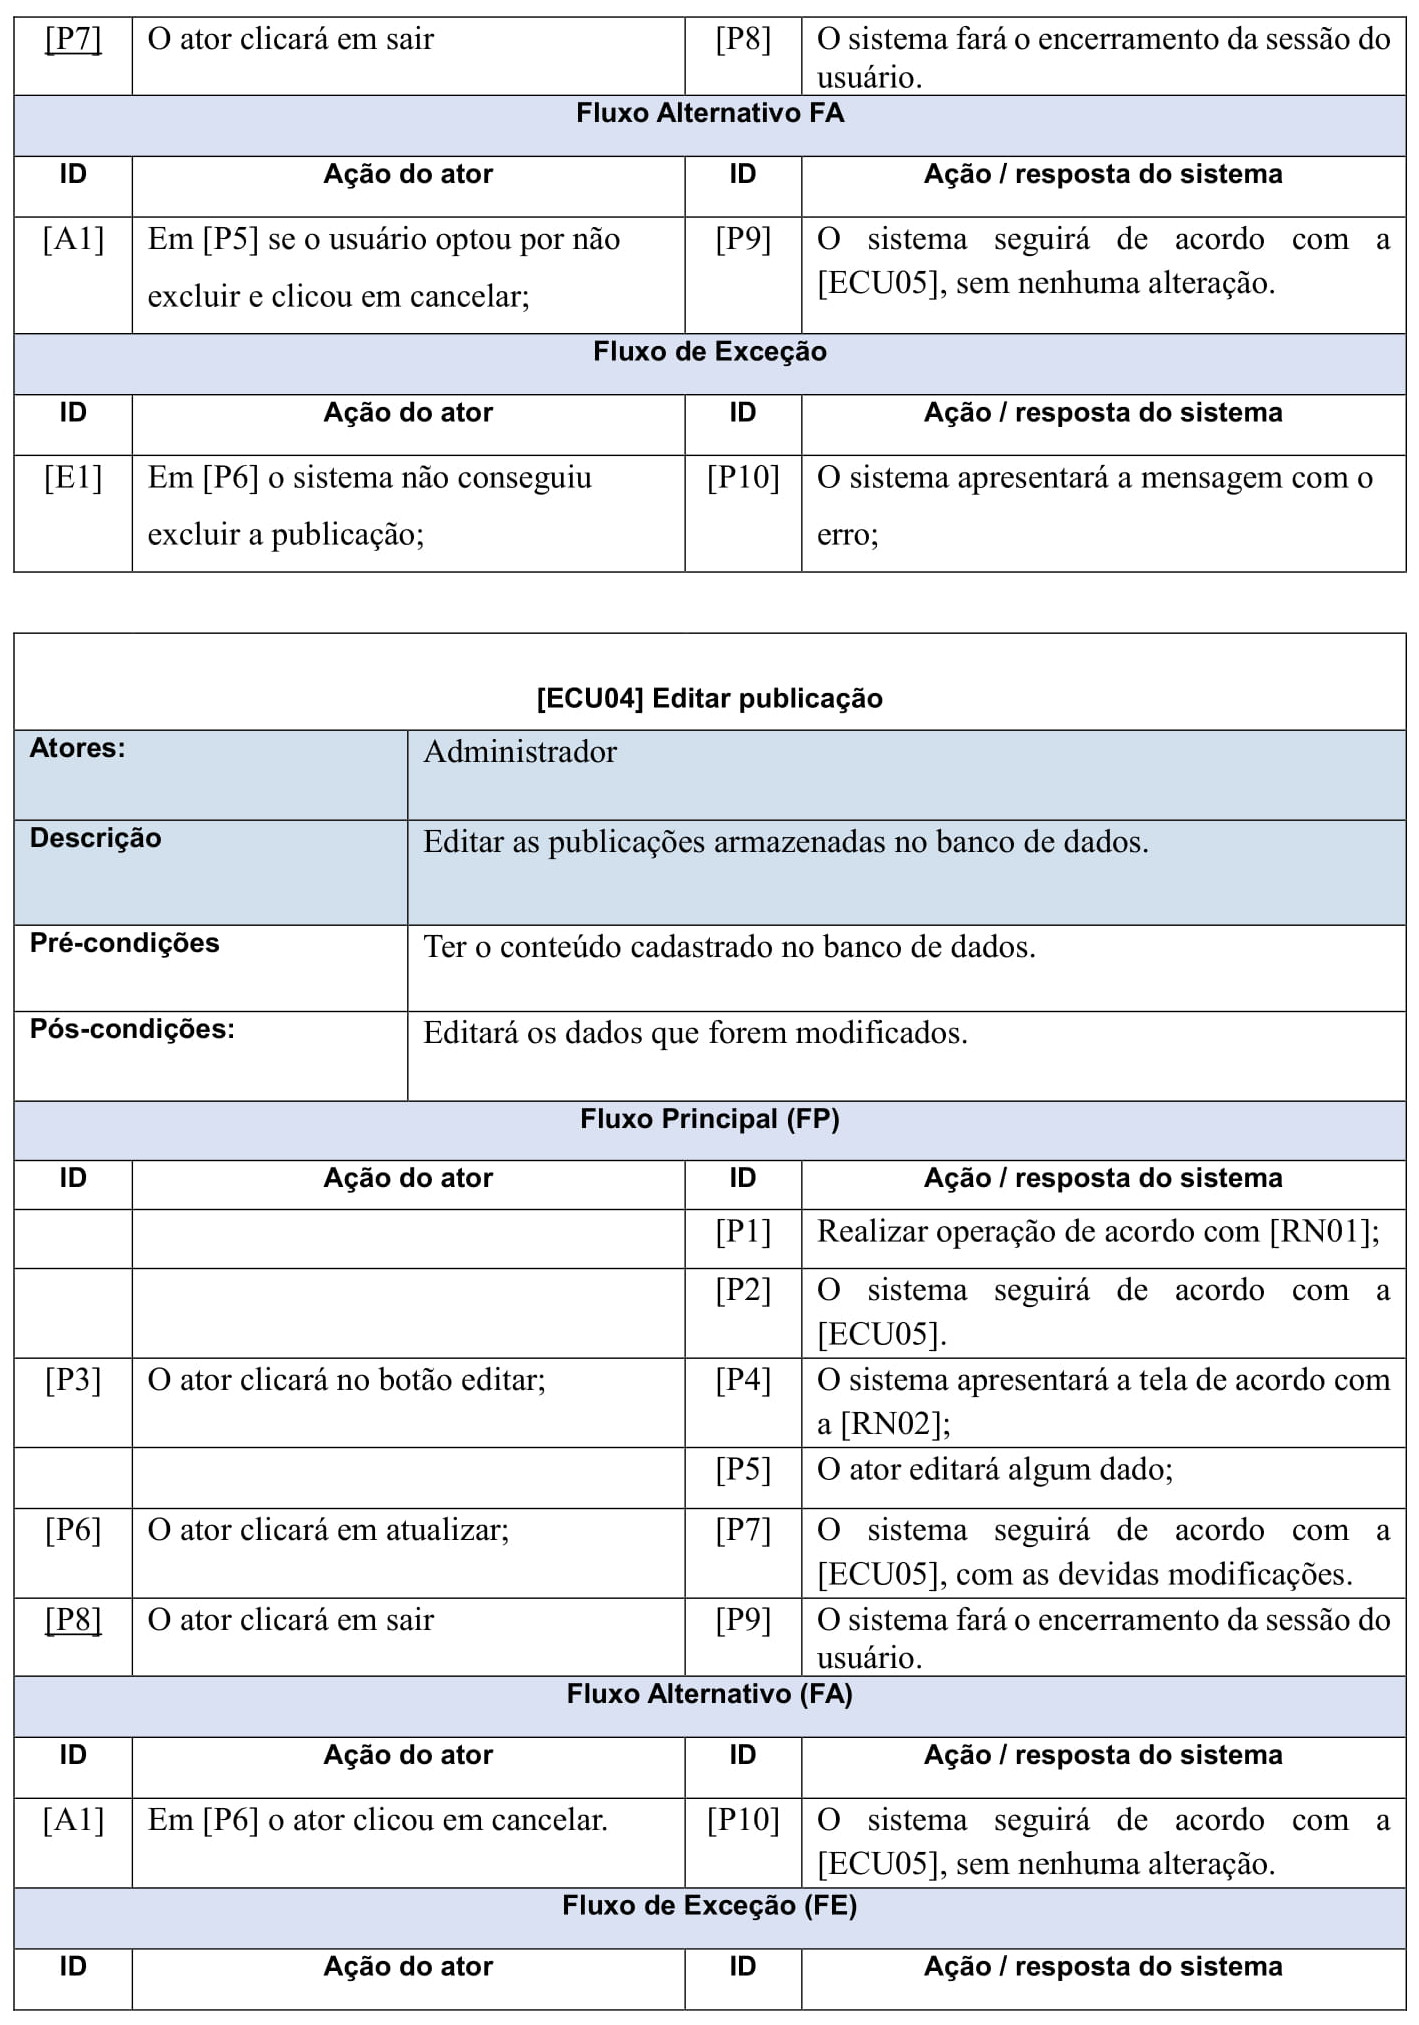
\includegraphics[width=\textwidth]{documentacao/ModeloArtefatos-08.jpg}
\end{figure}

\begin{figure}
    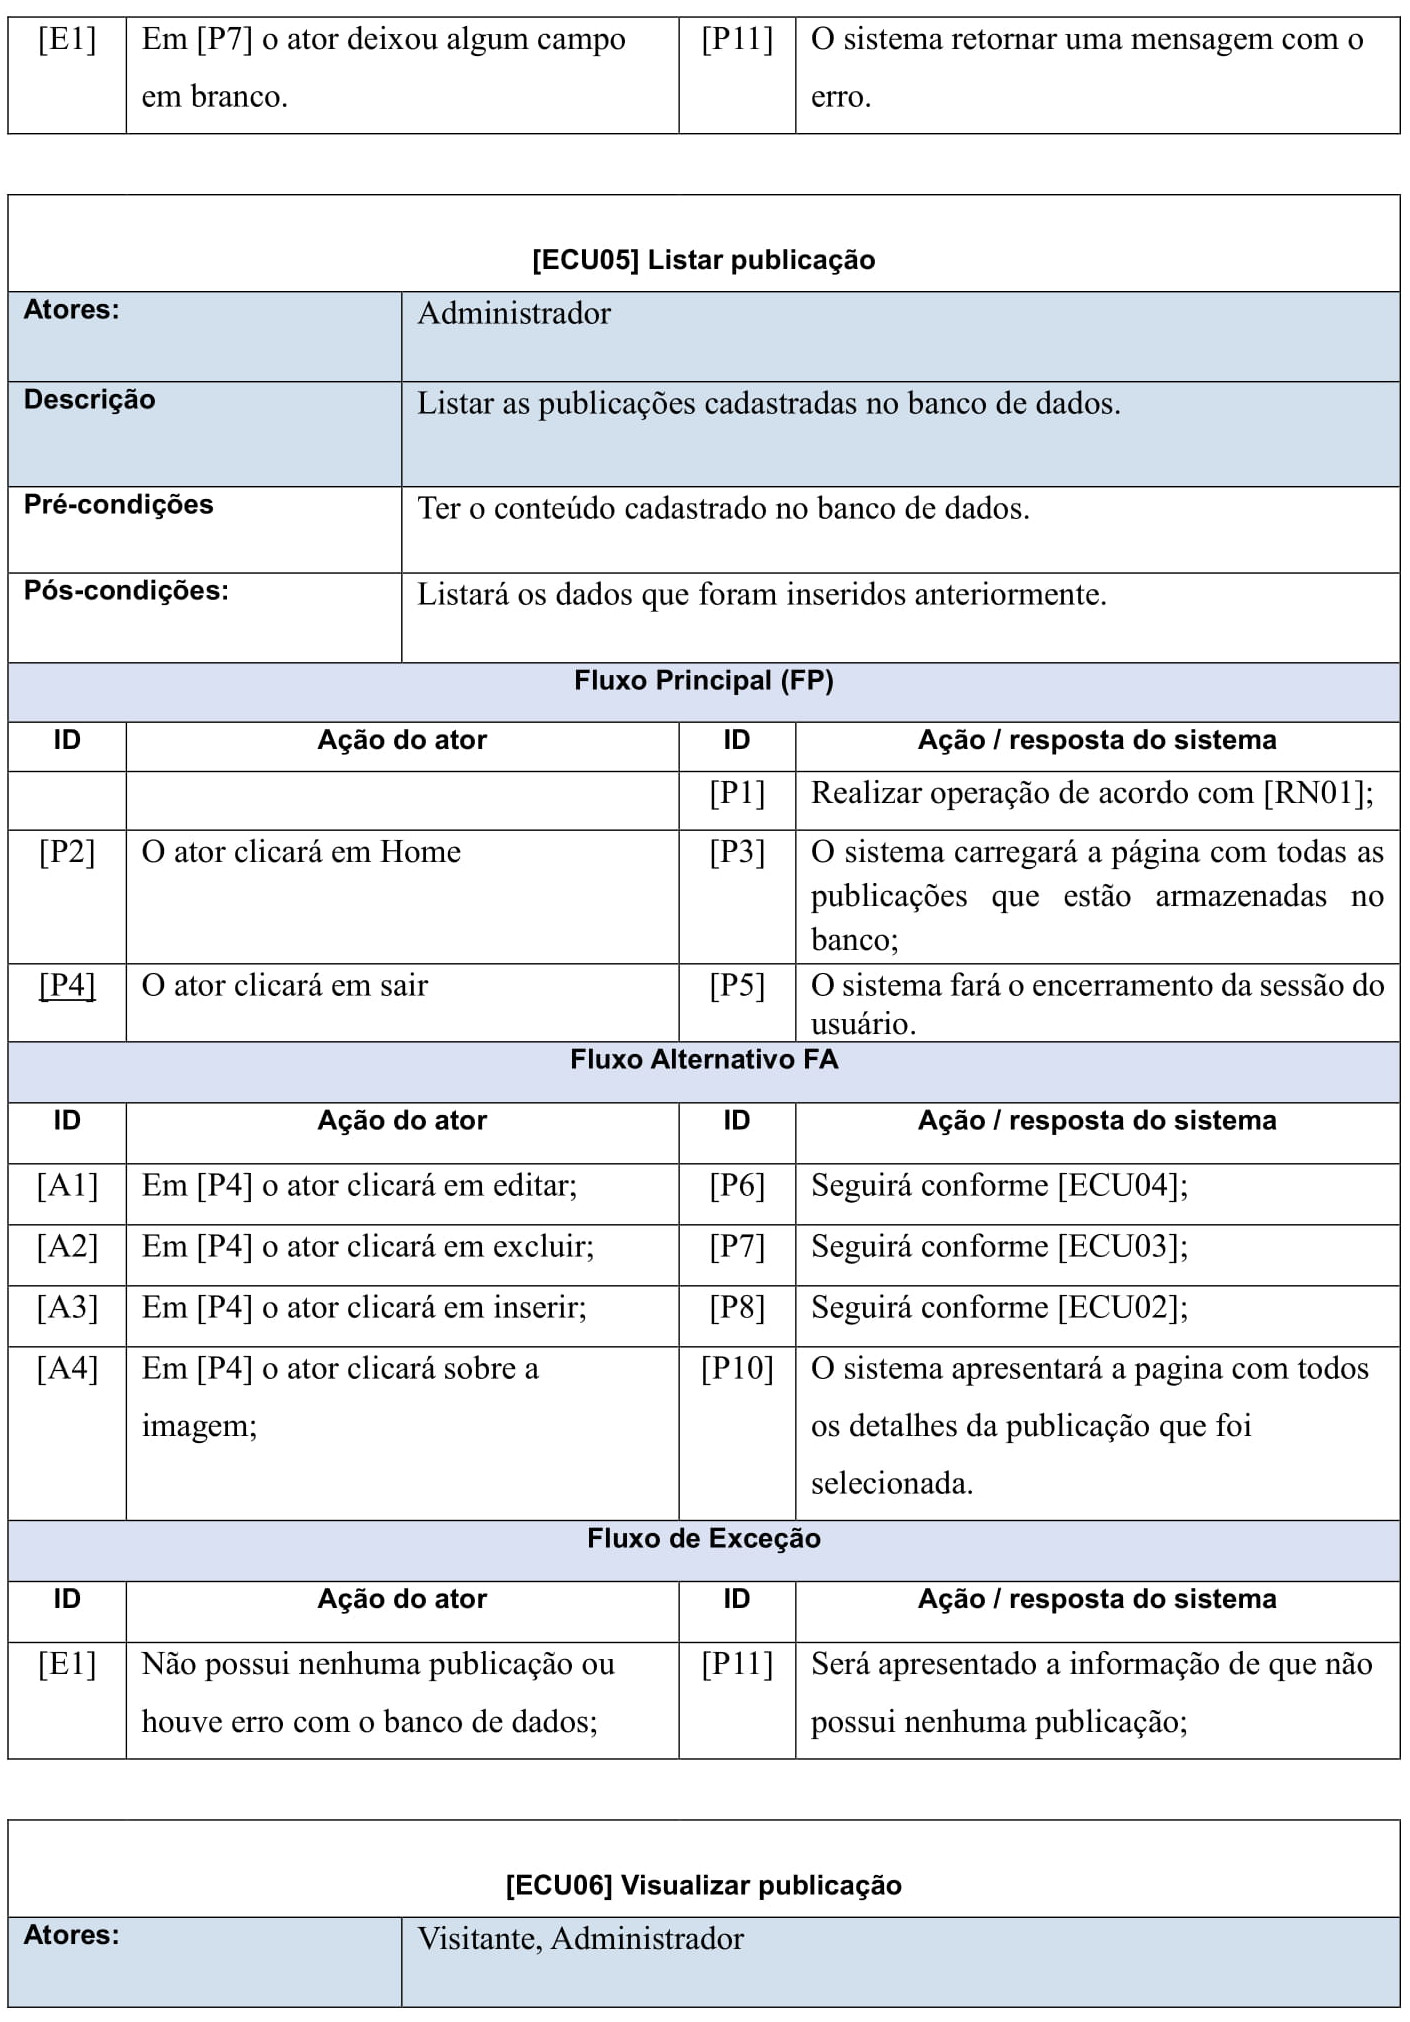
\includegraphics[width=\textwidth]{documentacao/ModeloArtefatos-09.jpg}
\end{figure}

\begin{figure}[H]
    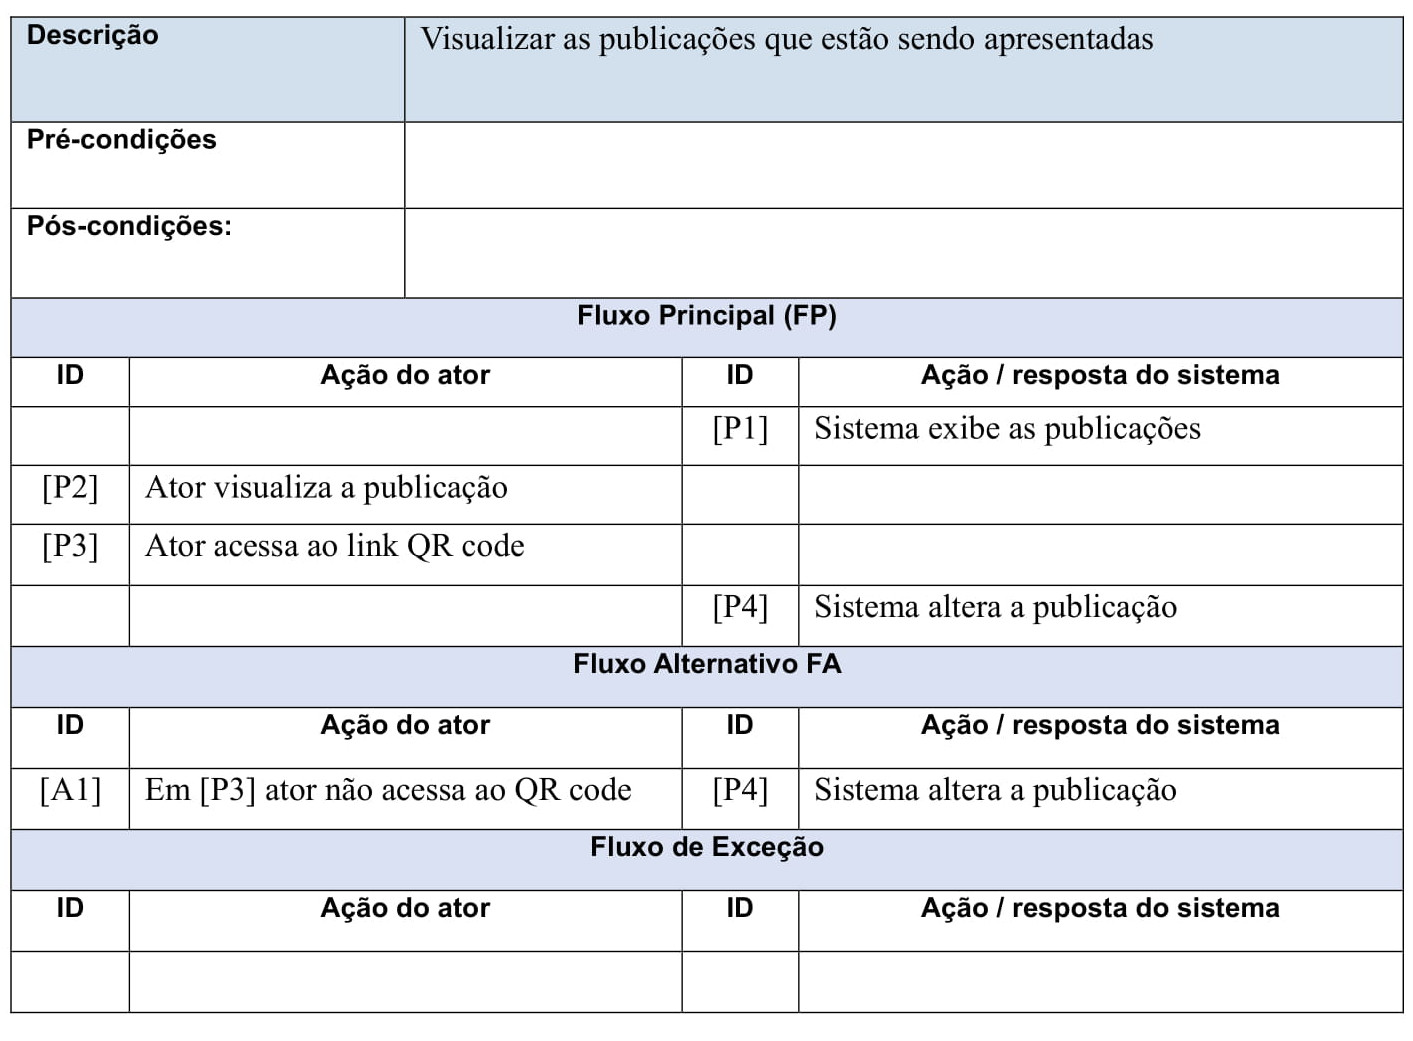
\includegraphics[width=\textwidth]{documentacao/ModeloArtefatos-10.jpg}
\end{figure}

